\section{\uppercase{Results}}
\label{sec:resul}

\noindent Results presented here originated from one of three machines, that will be referred to as Alpha, Bravo and Charlie.
The main specifications of each machine are as follows:
\begin{itemize}
  \item \textbf{Alpha}: 4 GBs of main memory, a 2 core Intel i3-2310M 2.1GHz CPU and a NVIDIA GT520M with 1 GB;
  \item \textbf{Bravo}: 32 GBs of main memory, a 6 core Intel i7-4930K 3.4GHz CPU and a NVIDIA Quadro K600 with 1 GB;
  \item \textbf{Charlie}: 32 GBs of main memory, a 4 core Intel i7-4770K 3.5GHz CPU and a NVIDIA K40c with 12 GB.
\end{itemize}

%%%%%%%%%%%%%%%%%%%%%%%%%%%%%%%%%%%%%%%%%%%%%%%%%%%%%%%%%%%%%%%%%%%%%%
\subsection{GPU Parallel K-Means}

\noindent Both sequential and parallel versions of K-Means were executed over a wide spectrum of datasets varying number of patterns, features and centroids.
All tests were executed on machine Charlie and the block size was maintained constant at 512.
%Whenever the number of clusters was superior to $70\%$ of the number of patterns (e.g. 800 clusters for a dataset with 1000 pattern), that particular test case was not executed.
The sequential version used a single thread.

Observing Figures \ref{fig:kmeans dims}A and \ref{fig:kmeans dims}B, it is clear that the number of patterns, features and clusters influence the speed-up.
For the simple case of 2 dimensions (Fig \ref{fig:kmeans dims}A), the speed-up increases with the number of patterns.
However, there is no speed-up when the overall complexity of the datasets is low.
% For 2 clusters, there is no speed-up before $100 \: 000$ patterns.
% And even after that mark, the speed-up is not significant.
% On the other hand, for a large number of clusters, there is speed-up for any number of patterns executed.
% Not only that, that speed-up is highest for a superior number of clusters.
As the complexity of the problem increases (more centroids and patterns), the speed-up also increases.
The reason for this is that the total amount of work increases linearly with the number of clusters but is diluted by the number of threads that can execute simultaneously.

\begin{figure}[hbtp]
    \centering
    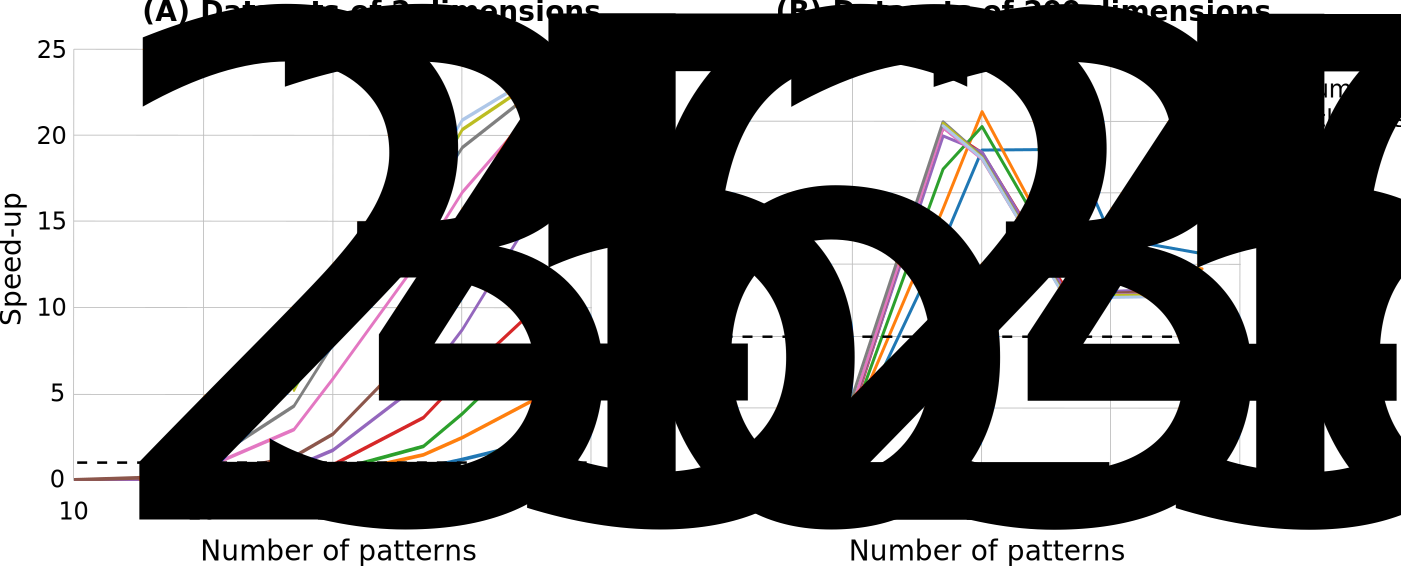
\includegraphics[width=\columnwidth]{speedup_dim}
    \caption{Speed-up of the labeling phase for datasets of 2 dimensions and varying the number of patterns and clusters. The dotted black line represents a speed-up of one.}
    \label{fig:kmeans dims}
\end{figure}

As the dimensionality increases (Fig. \ref{fig:kmeans dims}B), the speed-up increases until a certain number of patterns and then decreases.
Here, the initial number of patterns for which there is a speed-up is lower and the number of clusters plays less an influence on the speed-up.
We believe the reason for this is related to the implementation itself.
The current parallel implementation does not use shared memory, which is fast.
As such, for every computation, each thread fetches the relevant data from global memory which is significantly slower.
As the number of dimensions increases, the amount of data that each thread must fetch also increases.
Furthermore, since the number of dimensions affects both data points and centroids, if the number of dimensions increases by 2 the number of fetches to memory increases by 4.
So, the speed-up increases with the dataset complexity until a point where the number of fetches to memory starts having a very significant effect on the execution time and it decreases close to $50\%$.

%%%%%%%%%%%%%%%%%%%%%%%%%%%%%%%%%%%%%%%%%%%%%%%%%%%%%%%%%%%%%%%%%%%%%%
\subsection{Validation with original}

\noindent The results of the original version of EAC, implemented in Matlab, are compared with those of the proposed solution.
Several small datasets, chosen from the datasets used in \cite{Lourenco2010} and taken from the UCI Machine Learning repository \cite{Lichman:2013}, were processed by the two versions of EAC.
Both versions are processed from the same ensembles since production is probabilistic, which guarantees that the combination and recovery phases are equivalent.
% Furthermore, since the generation of the ensemble is probabilistic and can change the results between runs, the proposed version is processed with the ensembles created by the original version as well.
% This guarantees that the combination and recovery phases of EAC, which are deterministic when using SL, are equivalent to the original.
All processing was done in machine Alpha.
% All data in this section refers to processing done in machine Alpha.
Table \ref{tab:validation error acc} presents the difference between the accuracies of the two versions.
% Analyzing these results, it is apparent that the difference is minimal, most likely due the original version using Matlab and the proposed using Python.
It's clear the difference is minimal, most likely due the original version using Matlab and the proposed using Python. 
Moreover, a speed-up as low as 6 and as high as 200 was obtained over the original version in the various steps.%, including the production step.

\begin{table}[h]
\centering
\caption{Difference between accuracy of the two implementations of EAC, using the same ensemble. Accuracy was measured using the H-index \cite{Meila2003}.}

\begin{tabular}{lll}
\toprule
         &        \multicolumn{2}{c}{Number of clusters scheme} \\
Dataset &      Fixed & Lifetime \\
\midrule
breast\_cancer &  4.94e-06 &     2.82e-06 \\
ionosphere     &  1.65e-06 &     1.45e-06 \\
iris           &  3.33e-06 &     3.33e-06 \\
isolet         &  1.03e-07 &     4.08e-07 \\
optdigits      &  3.79e-06 &     1.48e-06 \\
pima           &  3.33e-06 &     3.33e-06 \\
pima\_norm     &  4.16e-07 &     4.16e-07 \\
wine\_norm     &  1.12e-07 &     1.91e-06 \\
\bottomrule
\end{tabular}

\label{tab:validation error acc}
\end{table}

%%%%%%%%%%%%%%%%%%%%%%%%%%%%%%%%%%%%%%%%%%%%%%%%%%%%%%%%%%%%%%%%%%%%%%
\subsection{Large dataset testing}

\noindent This section presents results referring to a large dataset comprised by a mixture of 6 Gaussians, where 2 pairs are overlapped and 1 pair is touching.
% The results here presented refer to a synthetic large dataset comprised by a mixture of 6 Gaussians, where 2 pairs are overlapped and 1 pair is touching.
This dataset was sampled into smaller datasets to analyze different dataset sizes.

Different rules for computing the $K_{min}$, different co-association matrix formats and different approaches for the final clustering will be mentioned.
The different rules are presented in Table \ref{tab:eac rules}.
The different co-association matrix formats are the \emph{full} (for fully allocated $n \times n$ matrix), \emph{full condensed} (for a fully allocated $\frac{n(n-1)}{2}$ array to build the upper triangular matrix), \emph{sparse complete} (for EAC CSR), \emph{sparse condensed const} (for EAC CSR building only the upper triangular matrix) and \emph{sparse condensed linear} (for EAC CSR condensed).
The different approaches for the final clustering are \emph{SLINK} \cite{Sibson1973}, \emph{SL-MST} (for using the Kruskal implementation in SciPy) and \emph{SL-MST-Disk} for disk-based variant.

\begin{table}[h]
\centering
\caption{Different rules for computing $K_{min}$ and $K_{max}$. $n$ is the number of patterns and $sk$ is the number of patterns per cluster.}

\begin{tabular}{lcc}
\toprule
Rule &  $K_{min}$ &  $K_{max}$ \\
\midrule
\emph{sqrt}     & $\frac{\sqrt{n}}{2}$      & $\sqrt{n}$    \\
\emph{2sqrt}    & $\sqrt{n}$                & $2 \sqrt{n}$  \\
\emph{sk=sqrt2} & $sk = \frac{\sqrt{n}}{2}$ & $1.3 K_{min}$ \\
\emph{sk=300}   & $sk = 300$                & $1.3 K_{min}$ \\
\bottomrule
\end{tabular}

\label{tab:eac rules}
\end{table}

%changed
% The experiment that generated the results of these section was set up as follows.
% A large dataset was generated.
% The dataset was sampled uniformly to produce a smaller dataset with the desired number of patterns.
A clustering ensemble was produced (production phase) for each of these smaller datasets and for each of the rules. %, using K-Means. %changed
From each ensemble, co-association matrices were built.
A matrix format was not applicable when the dataset complexity would make the co-association matrix too big to fit in main memory.
The final clustering was also done for each of the matrix formats. %changed
The number of clusters was chosen with the lifetime criteria \cite{Fred2005}.
SL-MST was not executed if its space complexity was too big to fit in main memory. %changed
Furthermore, the combination and recovery phases were repeated several times, so as to make the influence of any background process less salient. %changed
For big datasets, the execution times are big enough that the influence of background processes is negligible. %changed
All processing was done in machine Bravo. %changed
The same analysis was performed on a dataset with separated Gaussians, from which similar conclusions were drawn. %changed

\subsubsection{Execution times}

\noindent Execution times are related with the $K_{min}$ parameter, whose evolution is presented in Fig. \ref{fig:eac kmin evo}.
Rules \emph{sqrt}, \emph{2sqrt} and \emph{sk=sqrt2} never intersect but rule $sk=300$ intersects all of them, finishing with the highest $K_{min}$.
Observing Fig. \ref{fig:eac execution times}A, one can see that the same thing happens to the production execution time associated with the $sk=300$ rule and the inverse happens to the combination time (Fig. \ref{fig:eac execution times}B).
A higher $K_{min}$ means more centroids for each K-Means run to compute, so it is not surprising that the execution time for computing the ensemble increases as $K_{min}$ increases.

\begin{figure}[hbt!]
    \centering
    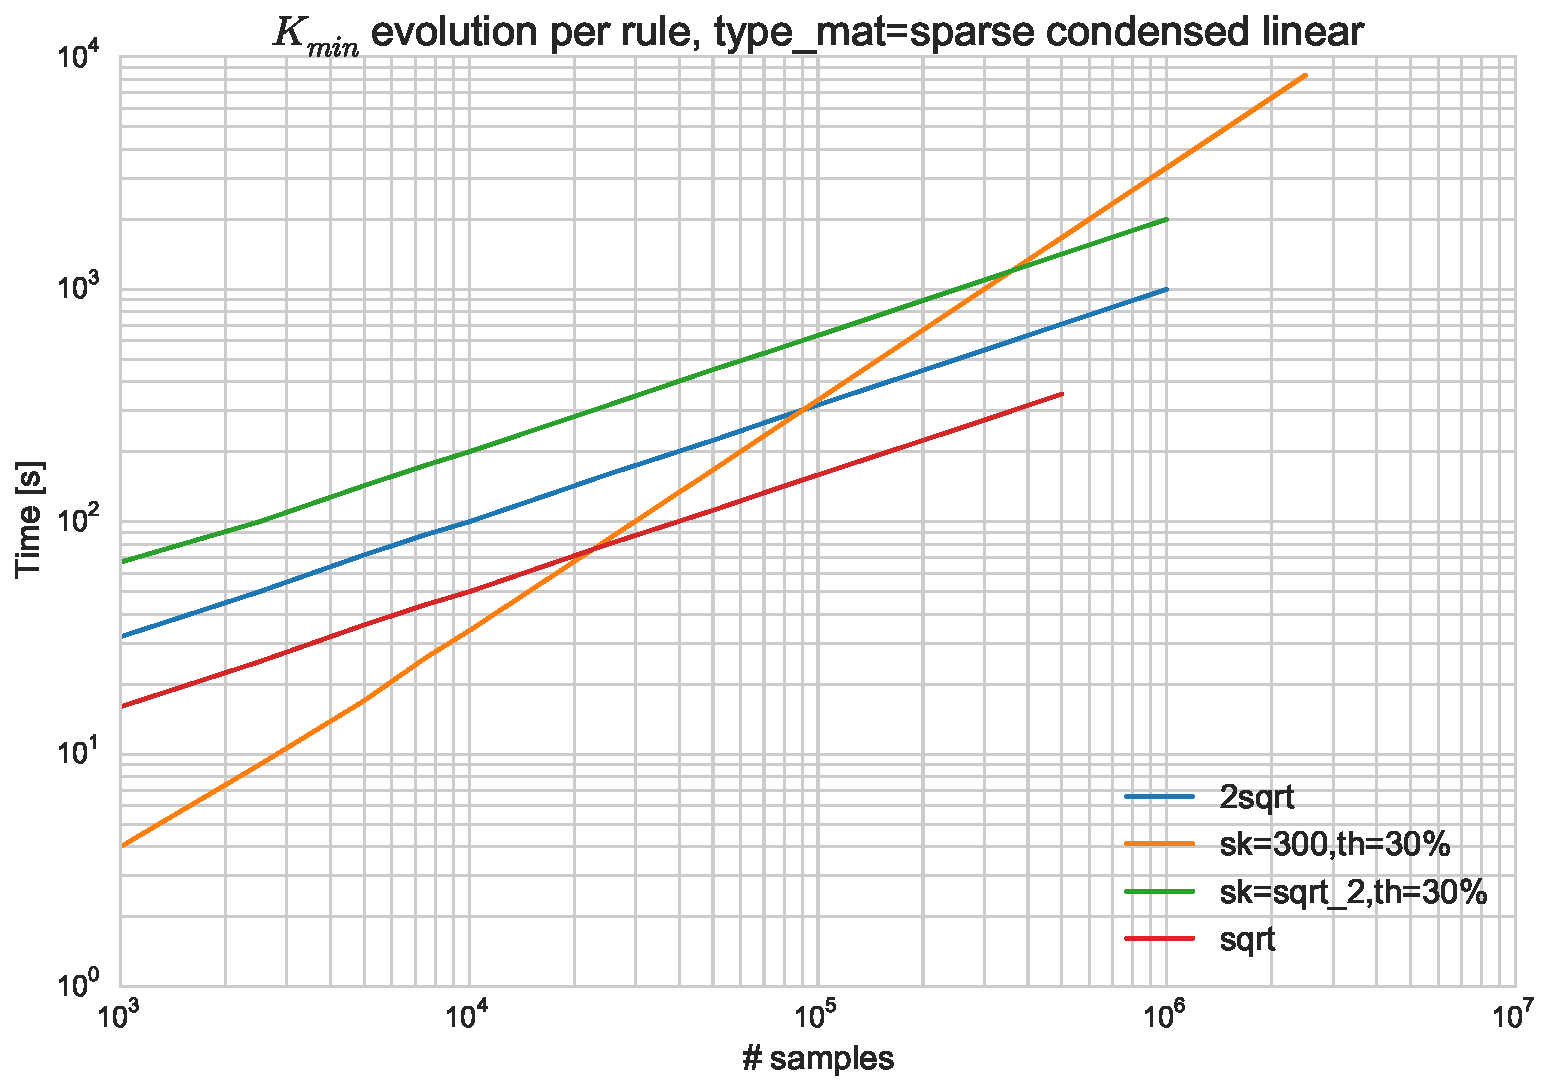
\includegraphics[width=0.55\columnwidth]{kmin_evolution}
    \caption{Evolution of $K_{min}$ with the number of patterns for different rules (type of matrix = sparse condensed linear).}
    \label{fig:eac kmin evo}
\end{figure}

\begin{figure}[hbt!]
    \centering
    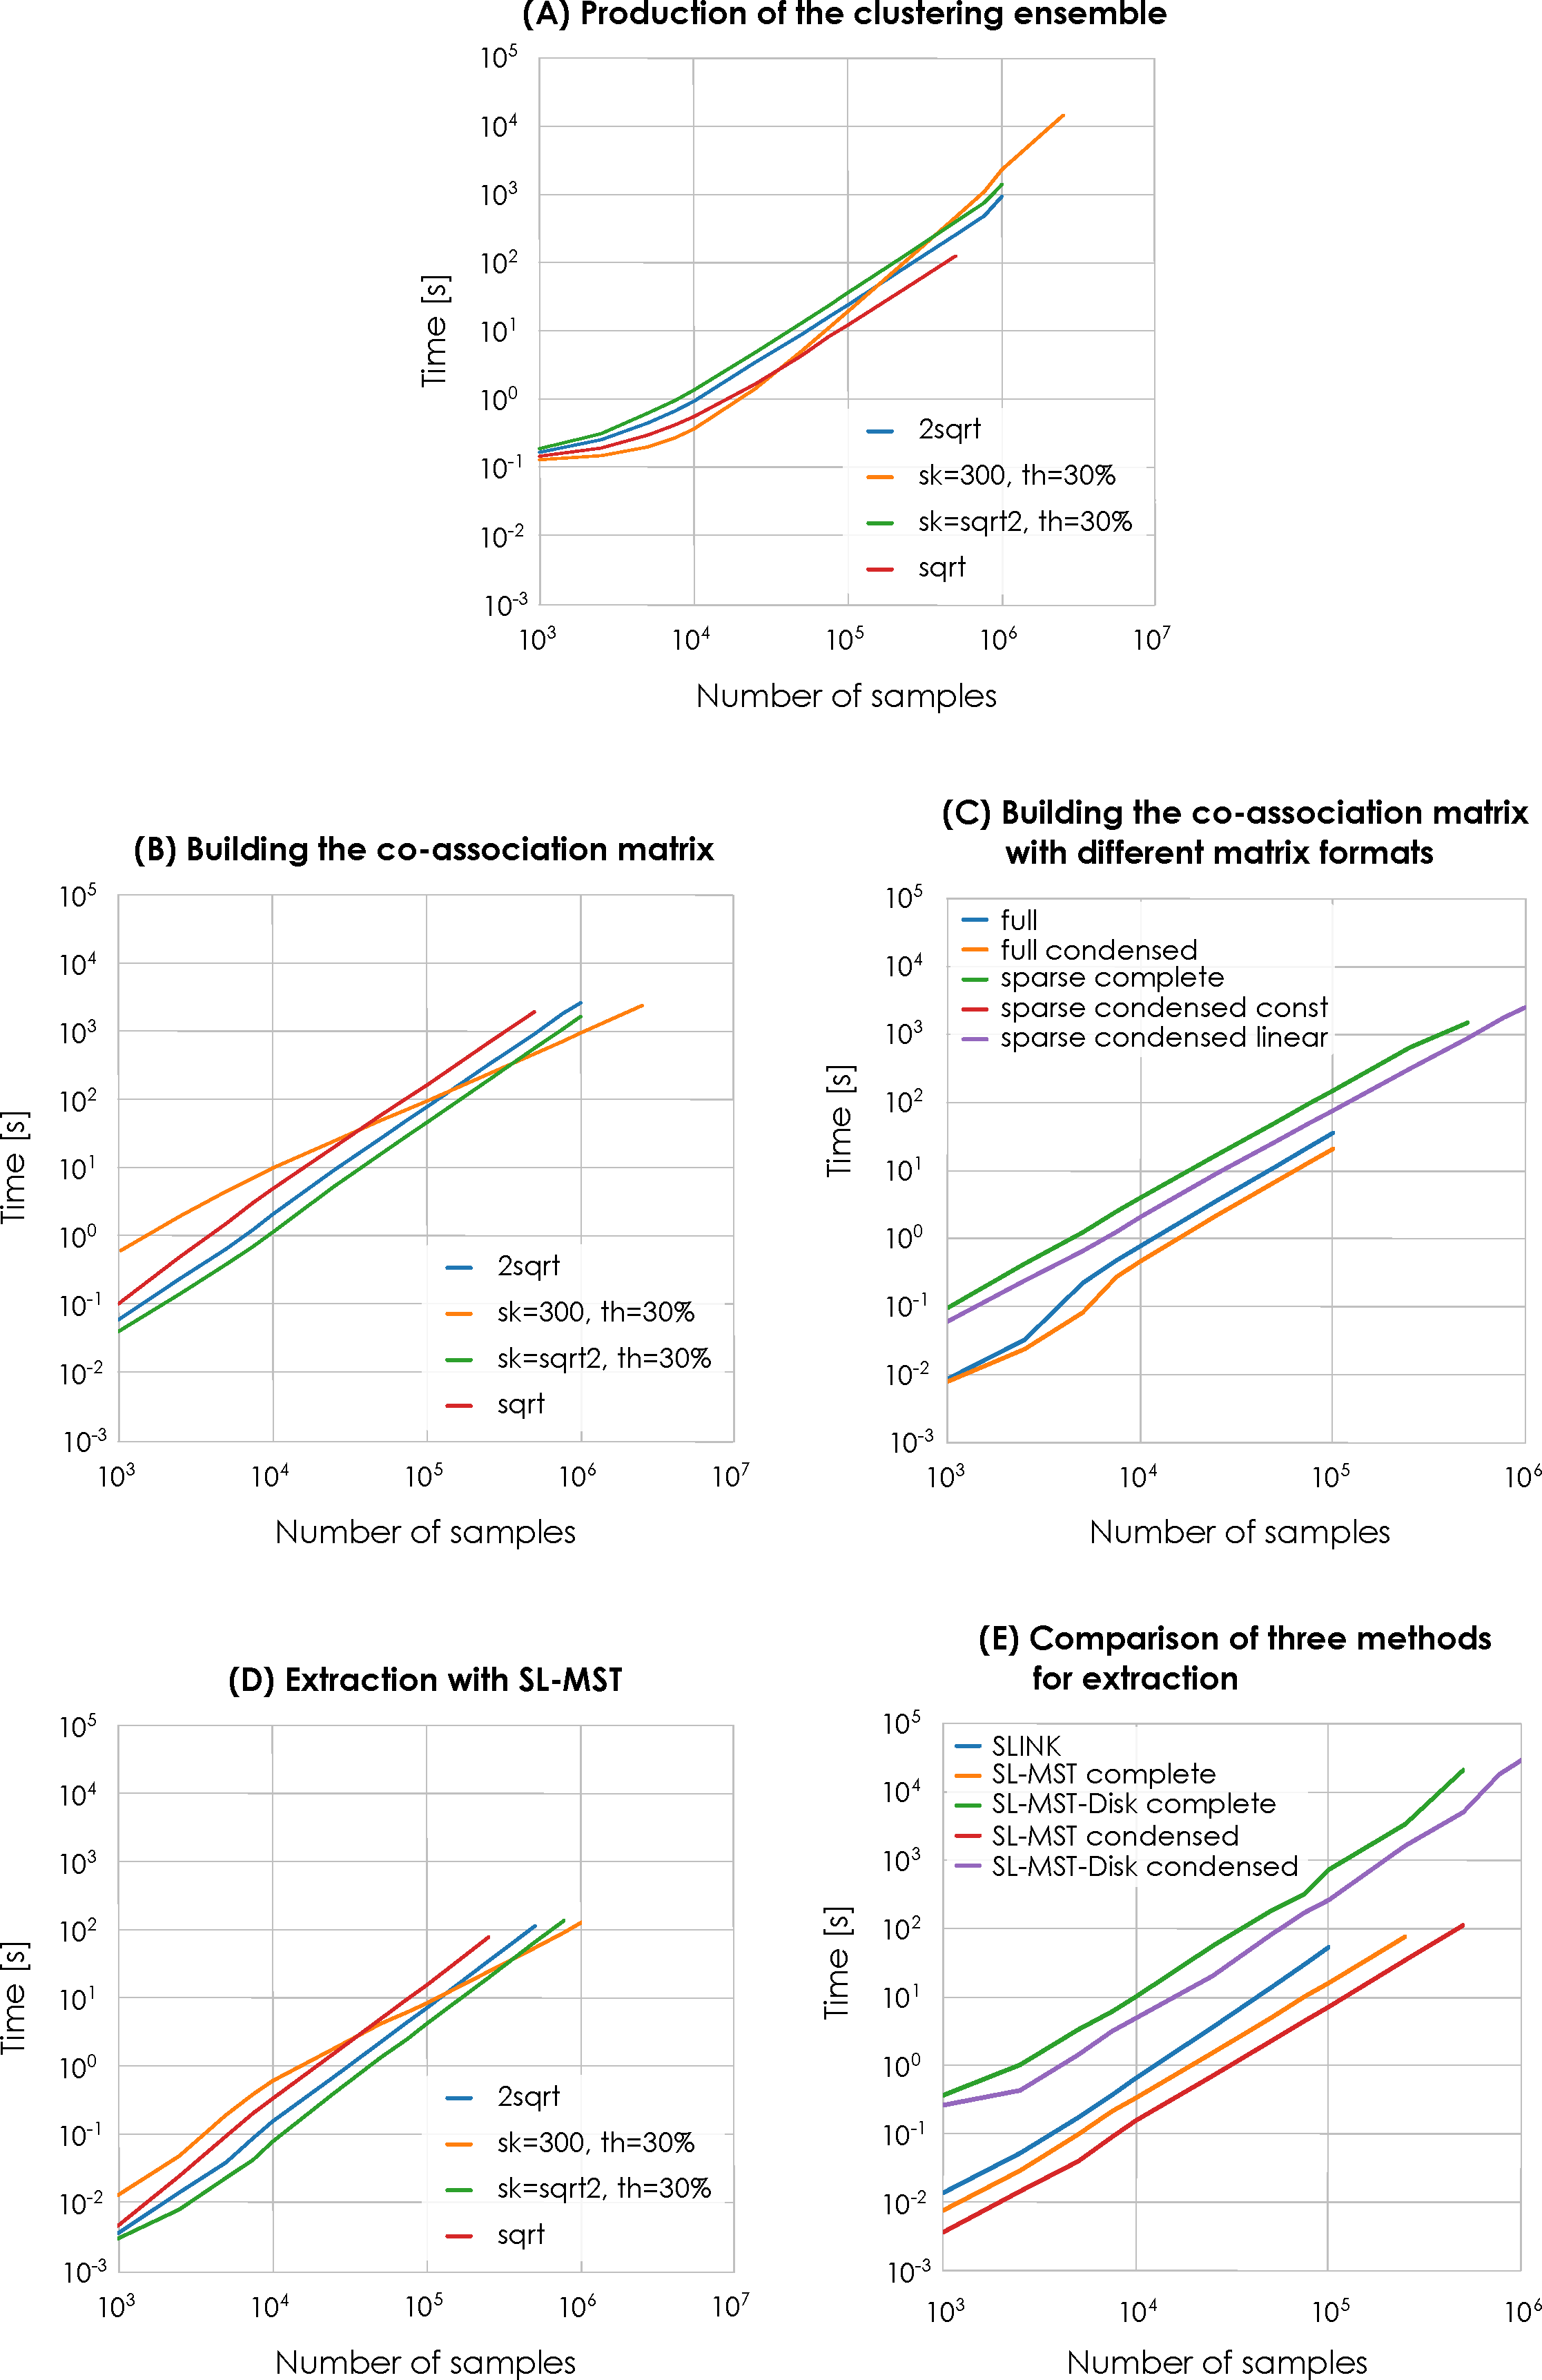
\includegraphics[width=\columnwidth]{execution_times}
    \caption{Execution time with different rules and variants for: (A) production of the clustering ensemble; (B,C) building the co-association matrix; and (D,E) extraction of the final partition with SL.}
%     \label{fig:eac execution times}
    \label{fig:eac execution times}
\end{figure}

% \begin{figure*}[hbt!]
%     \centering
%     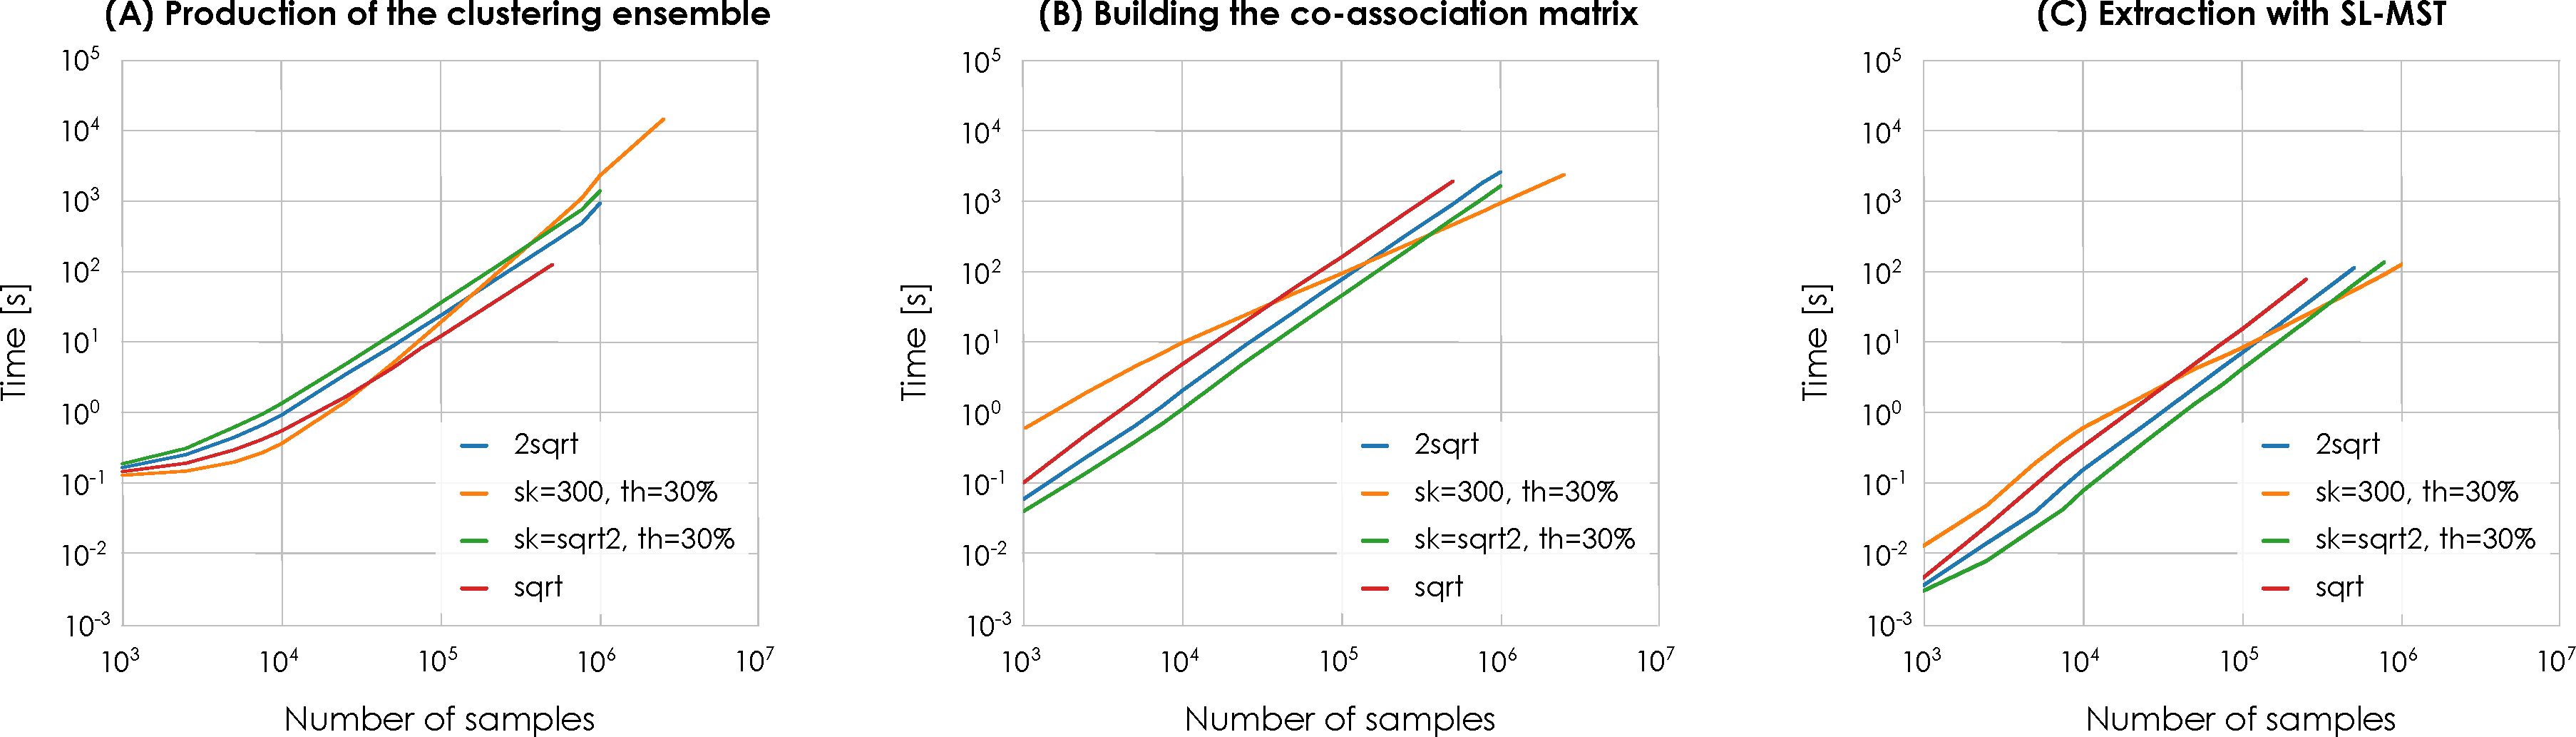
\includegraphics[width=0.8\textwidth]{execution_time_different_rules}
%     \caption{Execution time with different rules for: (A) production of the clustering ensemble; (B) building the co-association matrix; and (C) extraction of the final partition with SL-MST.}
%     \label{fig:eac execution times}
% \end{figure*}

Fig. \ref{fig:eac execution times}C shows the execution times on a longitudinal study for optimized matrix formats.
It is clear that the sparse formats are significantly slower than the fully allocated ones, specially for smaller datasets.
The \emph{full condensed} format usually takes around half the time than the \emph{full} format, since it performs half the operations. %changed
Idem for the \emph{sparse condensed} formats compared to the \emph{sparse complete}.
The big discrepancy between the sparse and full formats is due to the fact that the former needs to do a binary search at each association update and needs to keep the internal sparse data structure sorted.

The clustering times of the different methods of SL discussed previously (SLINK, SL-MST and SL-MST-Disk) are presented in Figures \ref{fig:eac execution times}D and \ref{fig:eac execution times}E.
The SL-MST-Disk method is significantly slower than any of the other methods.
This is expected, since it uses the hard drive which has very slow access times compared to main memory.
SL-MST is faster than SLINK, since it processes zero associations while SL-MST takes advantage of a graph representation and only processes the non-zero associations.
In resemblance to what happened with combination times, the condensed variants take roughly half the time has their complete counterparts, since SL-MST and SL-MST-Disk over condensed co-association matrices only process half the number of associations.
Although this is not depicted, SLINK takes roughly the same time for every rule, which means $K_{min}$ has no influence.
This comes as no surprise, since SLINK processes the whole matrix, regardless of its association sparsity.
The same rationale can be applied to SL-MST, where different rules can have significant influence over execution time, since they change the total number of associations.
As with the combination phase, the execution time referent to the \emph{sk=300} rule started with the greatest time and decreased as the number of patterns increased until it was the fastest. %changed

% new fig
% \begin{figure}[hbt!]
%     \centering
%     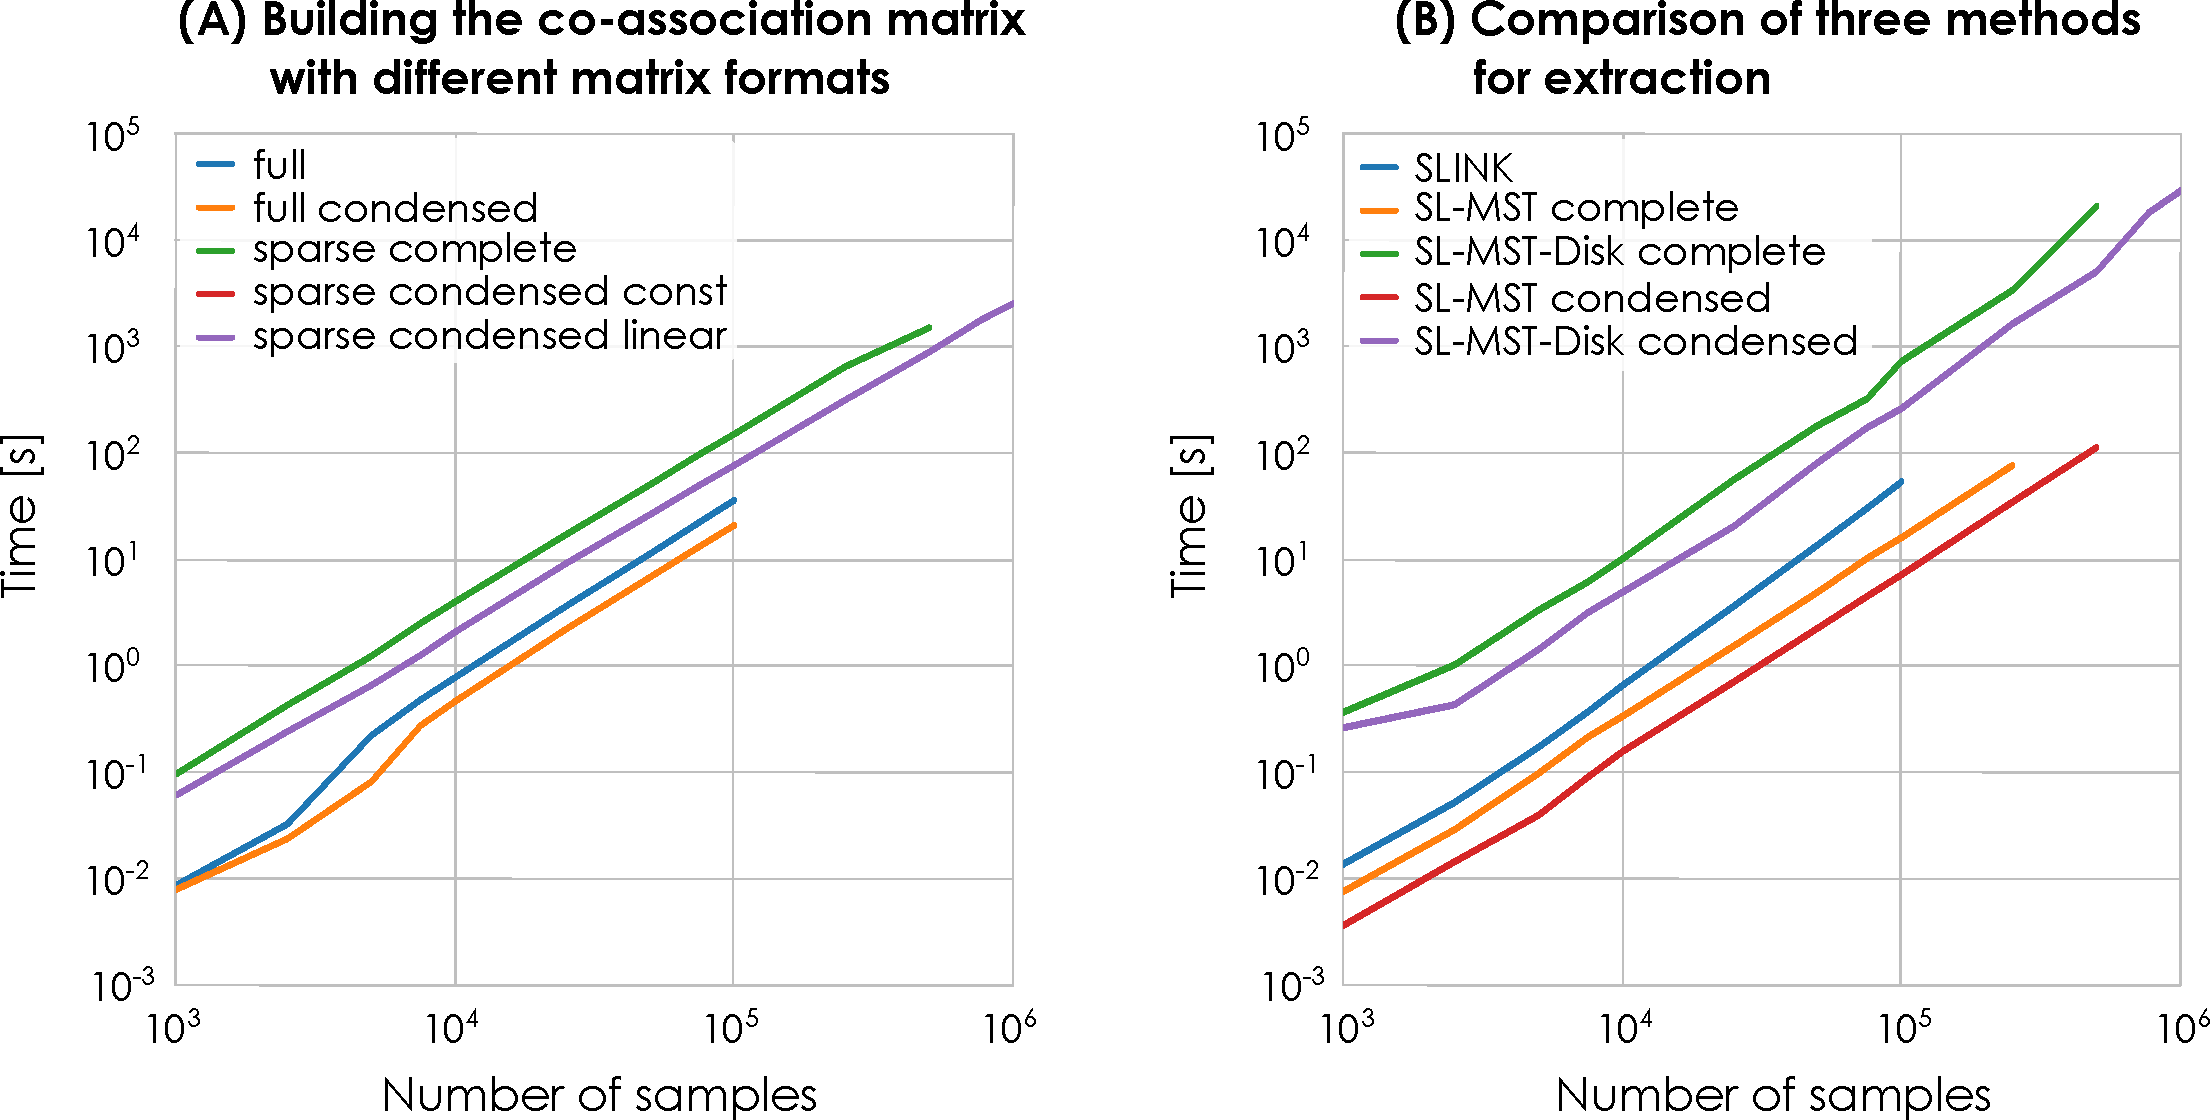
\includegraphics[width=\columnwidth]{matrix_formats_2sqrt}
%     \caption{Execution time with the rule 2sqrt for: (A) building the co-association matrix with different matrix formats; and (B) comparing three methods for extraction the final partition: SLINK runs over fully allocated condensed matrix while SL-MST and SL-MST-Disk run over the condensed and complete sparse matrices.}
%     \label{fig:eac sl}
% \end{figure}

The execution times of all phases combined are presented in Figures \ref{fig:eac total}A and \ref{fig:eac total}B.
The results are presented for the \emph{sparse condensed linear} format but the remaining results follow the same pattern.
It is interesting to note that, when using the SL-MST method in the recovery phase, the execution time for three of the rules do not differ much.
This is due to a sort of balancing between a slowing down of the production phase and a speeding up of the combination and recovery phases as the $K_{min}$ increases at a higher rate for $sk=300$ than for other rules.
This is not observed for the $sqrt$ rule as $K_{min}$ is always low enough that the total time is always dominated by the combination and recovery phases.
The same does not happen when using the SL-MST-Disk method, as the total time is completely dominated by the recovery phase.
This is clear, since the results in Fig. \ref{fig:eac total}B follow a pattern similar to that presented in Fig. \ref{fig:eac execution times}C.

% new fig
\begin{figure}[hbt!]
    \centering
    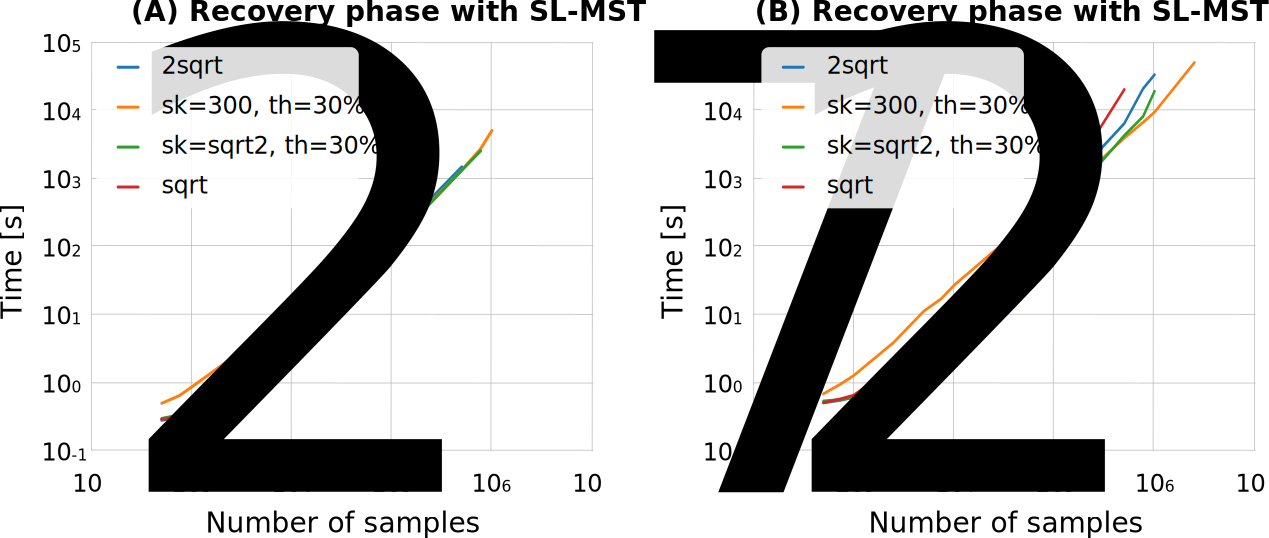
\includegraphics[width=\columnwidth]{total_execution_time}
    \caption{Execution times for all phases combined, using (A) SL-MST and (B) SL-MST-Disk in the recovery phase.}
    \label{fig:eac total}
\end{figure}

\subsubsection{Association density}

\noindent The sparse nature of EAC has been referred to before and is clearer in Fig. \ref{fig:eac assoc density}A.
This figure shows the association density, i.e. number of associations relative to the $n^2$ associations in a full matrix.
The \emph{full condensed} format has a constant density of $49.5\%$.
Idem for the \emph{sparse complete} and \emph{sparse condensed} formats, as long as no associations are discarded.
The overall tendency is for the density to decrease as the number of patterns of the dataset increases, since the \emph{full} matrix grows quadratically.
Besides, it would be expected that the same associations would be grouped together more frequently in partitions and simply make previous connections stronger instead of creating new ones, if the relationship between the number of patterns and $K_{min}$ is constant.

%new fig
\begin{figure}[hbt!]
    \centering
    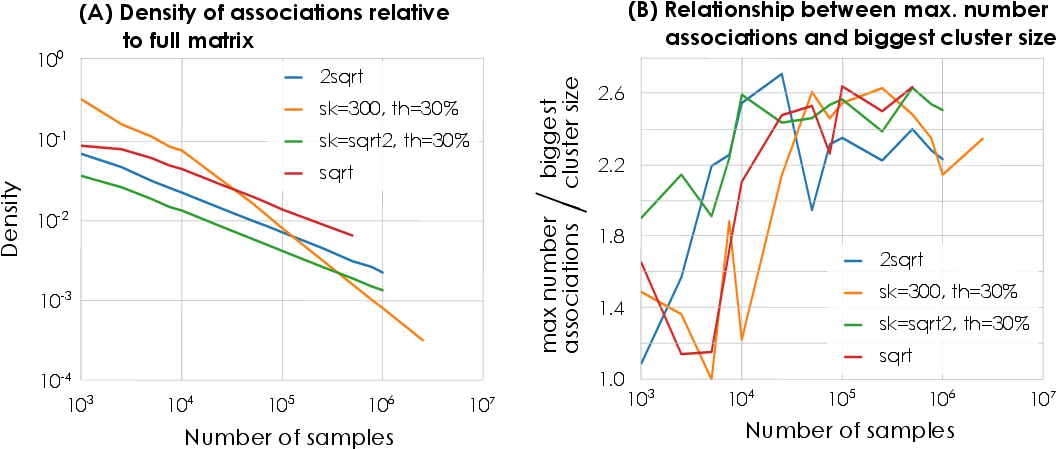
\includegraphics[width=\columnwidth]{assoc_density}
    \caption{(A) Density of associations relative to the full co-association matrix, which hold $n^2$ associations. (B) Maximum number of associations of any pattern divided by the number of patterns in the biggest cluster of the ensemble.}
    \label{fig:eac assoc density}
\end{figure}

Predicting the number of associations is useful for coming up with combination schemes that are both memory and speed efficient. %changed
% It was stated before that the biggest cluster size in any partition of the ensemble is a good parameter for this end.
Fig. \ref{fig:eac assoc density}B presents the ratio between the biggest cluster size and the maximum number of associations of any pattern.
These ratio increases with the number of patterns, but as the number of patterns increases it never goes over 3. %changed

However, the number of features of the used datasets is rather reduced.
It might be the case that this ratio would increase with the number of features, since there would be more degrees where the clusters might include other neighbors.
With this in mind, further studies ranging a wider spectrum of datasets should yield more enlightening conclusions or reinforce those presented here.

\subsubsection{Space complexity}

%new fig
\begin{figure}[hbt!]
    \centering
    \includegraphics[width=0.8\columnwidth]{{{sk_300}}}
    \caption{Memory used relative to the full $n^2$ matrix. The \emph{sparse complete} and \emph{sparse condensed const} curves are overlapped.}
    \label{fig:eac mem density}
\end{figure}

\noindent The allocated space for the space formats is based on a prediction that uses the biggest cluster size of the ensemble. %changed
This allocated space is usually more than what is necessary to store the total number of associations, to keep a safety margin.
Furthermore, the CSR sparse, on which the EAC CSR strategy is based, requires an array of the same size of the predicted number of associations. %changed
% This overhead may in fact make the sparse format pre-allocate more associations than are actually possible for some rules and in very small datasets.
Still, the allocated number of associations becomes a very small fraction compared to the \emph{full} matrix as the dataset complexity increases, which is the typical case for using a sparse format.
The actual memory used is presented in Fig. \ref{fig:eac mem density}.
The data types influence significantly the required memory. %changed
The associations can be stored in a single byte, since the number of partitions is usually less than 255.
This means that the memory used by the fully allocated formats is $n^2$ and $\frac{n(n-1)}{2}$ Bytes for the complete and condensed versions, respectively.
In the sparse formats, the values of the associations are also stored in an array of unsigned integers of 1 Byte.
However, an array of integers of 4 bytes of the same size must also be kept to keep track of the destination pattern each association belongs to.
One other array of integers of 8 bytes is kept but it is negligible compared to the other two arrays. %changed
The impact of the data types can be seen for smaller datasets where the total memory used is actually significantly higher than that of the \emph{full} matrix.
It should be noted that this discrepancy is not as high for other rules as for $sk=300$.
Still, the sparse formats, and in particular the condensed sparse format, are preferred since the memory used for large datasets is a small fraction of what would be necessary if using any of the fully allocated formats. %changed

